\section{Compte}

Dans cette section, il est expliqué comment créer un compte, gérer ce compte, et se connecter, et se déconnecter.

\subsection{Créer un compte}

Pour créer un compte utilisateur à partir de n'importe quelle page, cliquez sur le bouton "Inscription" proposé dans le menu spécial dans le coin en haut, à droite de l'écran, comme indiqué à la figure ci-dessous.

\begin{figure}[H]
\centering
\includegraphics[scale=0.15]{user_images/basic_user/GererConnexion/Senregistrer/001.jpg}
\caption{Création compte, étape 1}
\end{figure}

Ensuite, remplissez le formulaire pour créer un compte. Celui-ci est décomposé en 2 parties : la première concerne les informations importantes de connexion, et la deuxième partie concerne les informations personnelles de l'utilisateur. \newline

Les champs dont le nom est suivi par une étoile (*) doivent obligatoirement être remplis. Les autres champs sont optionnels.

\begin{figure}[H]
\centering
\includegraphics[scale=0.15]{user_images/basic_user/GererConnexion/Senregistrer/002.jpg}
\caption{Création compte, étape 2}
\end{figure}

Lorsque vous avez terminé de remplir le formulaire, vous pouvez cliquer sur le bouton "Inscription" en bas de la page, comme indiqué à la figure ci-dessous.

\begin{figure}[H]
\centering
\includegraphics[scale=0.15]{user_images/basic_user/GererConnexion/Senregistrer/003.jpg}
\caption{Création compte, étape 3}
\end{figure}

Si le formulaire est invalide, vous aurez un message indiquant précisément l'erreur. Dans le cas contraire, vous serez invités à consulter vos emails à l'adresse email que vous avez mis dans le formulaire, comme le montre l'image ci-dessous.

\begin{figure}[H]
\centering
\includegraphics[scale=0.15]{user_images/basic_user/GererConnexion/Senregistrer/004.jpg}
\caption{Création compte, étape 4}
\end{figure}

Vous pouvez accéder à la plupart des pages d'un utilisateur standard. Pour accéder pleinement à toutes les pages d'un utilisateur standard, vous devez obligatoirement valider votre adresse email. \newline

Dans votre boîte email, vous devriez avoir un email similaire à celui sur l'image ci-dessous. Un lien vous est proposé pour valider votre compte.

\begin{figure}[H]
\centering
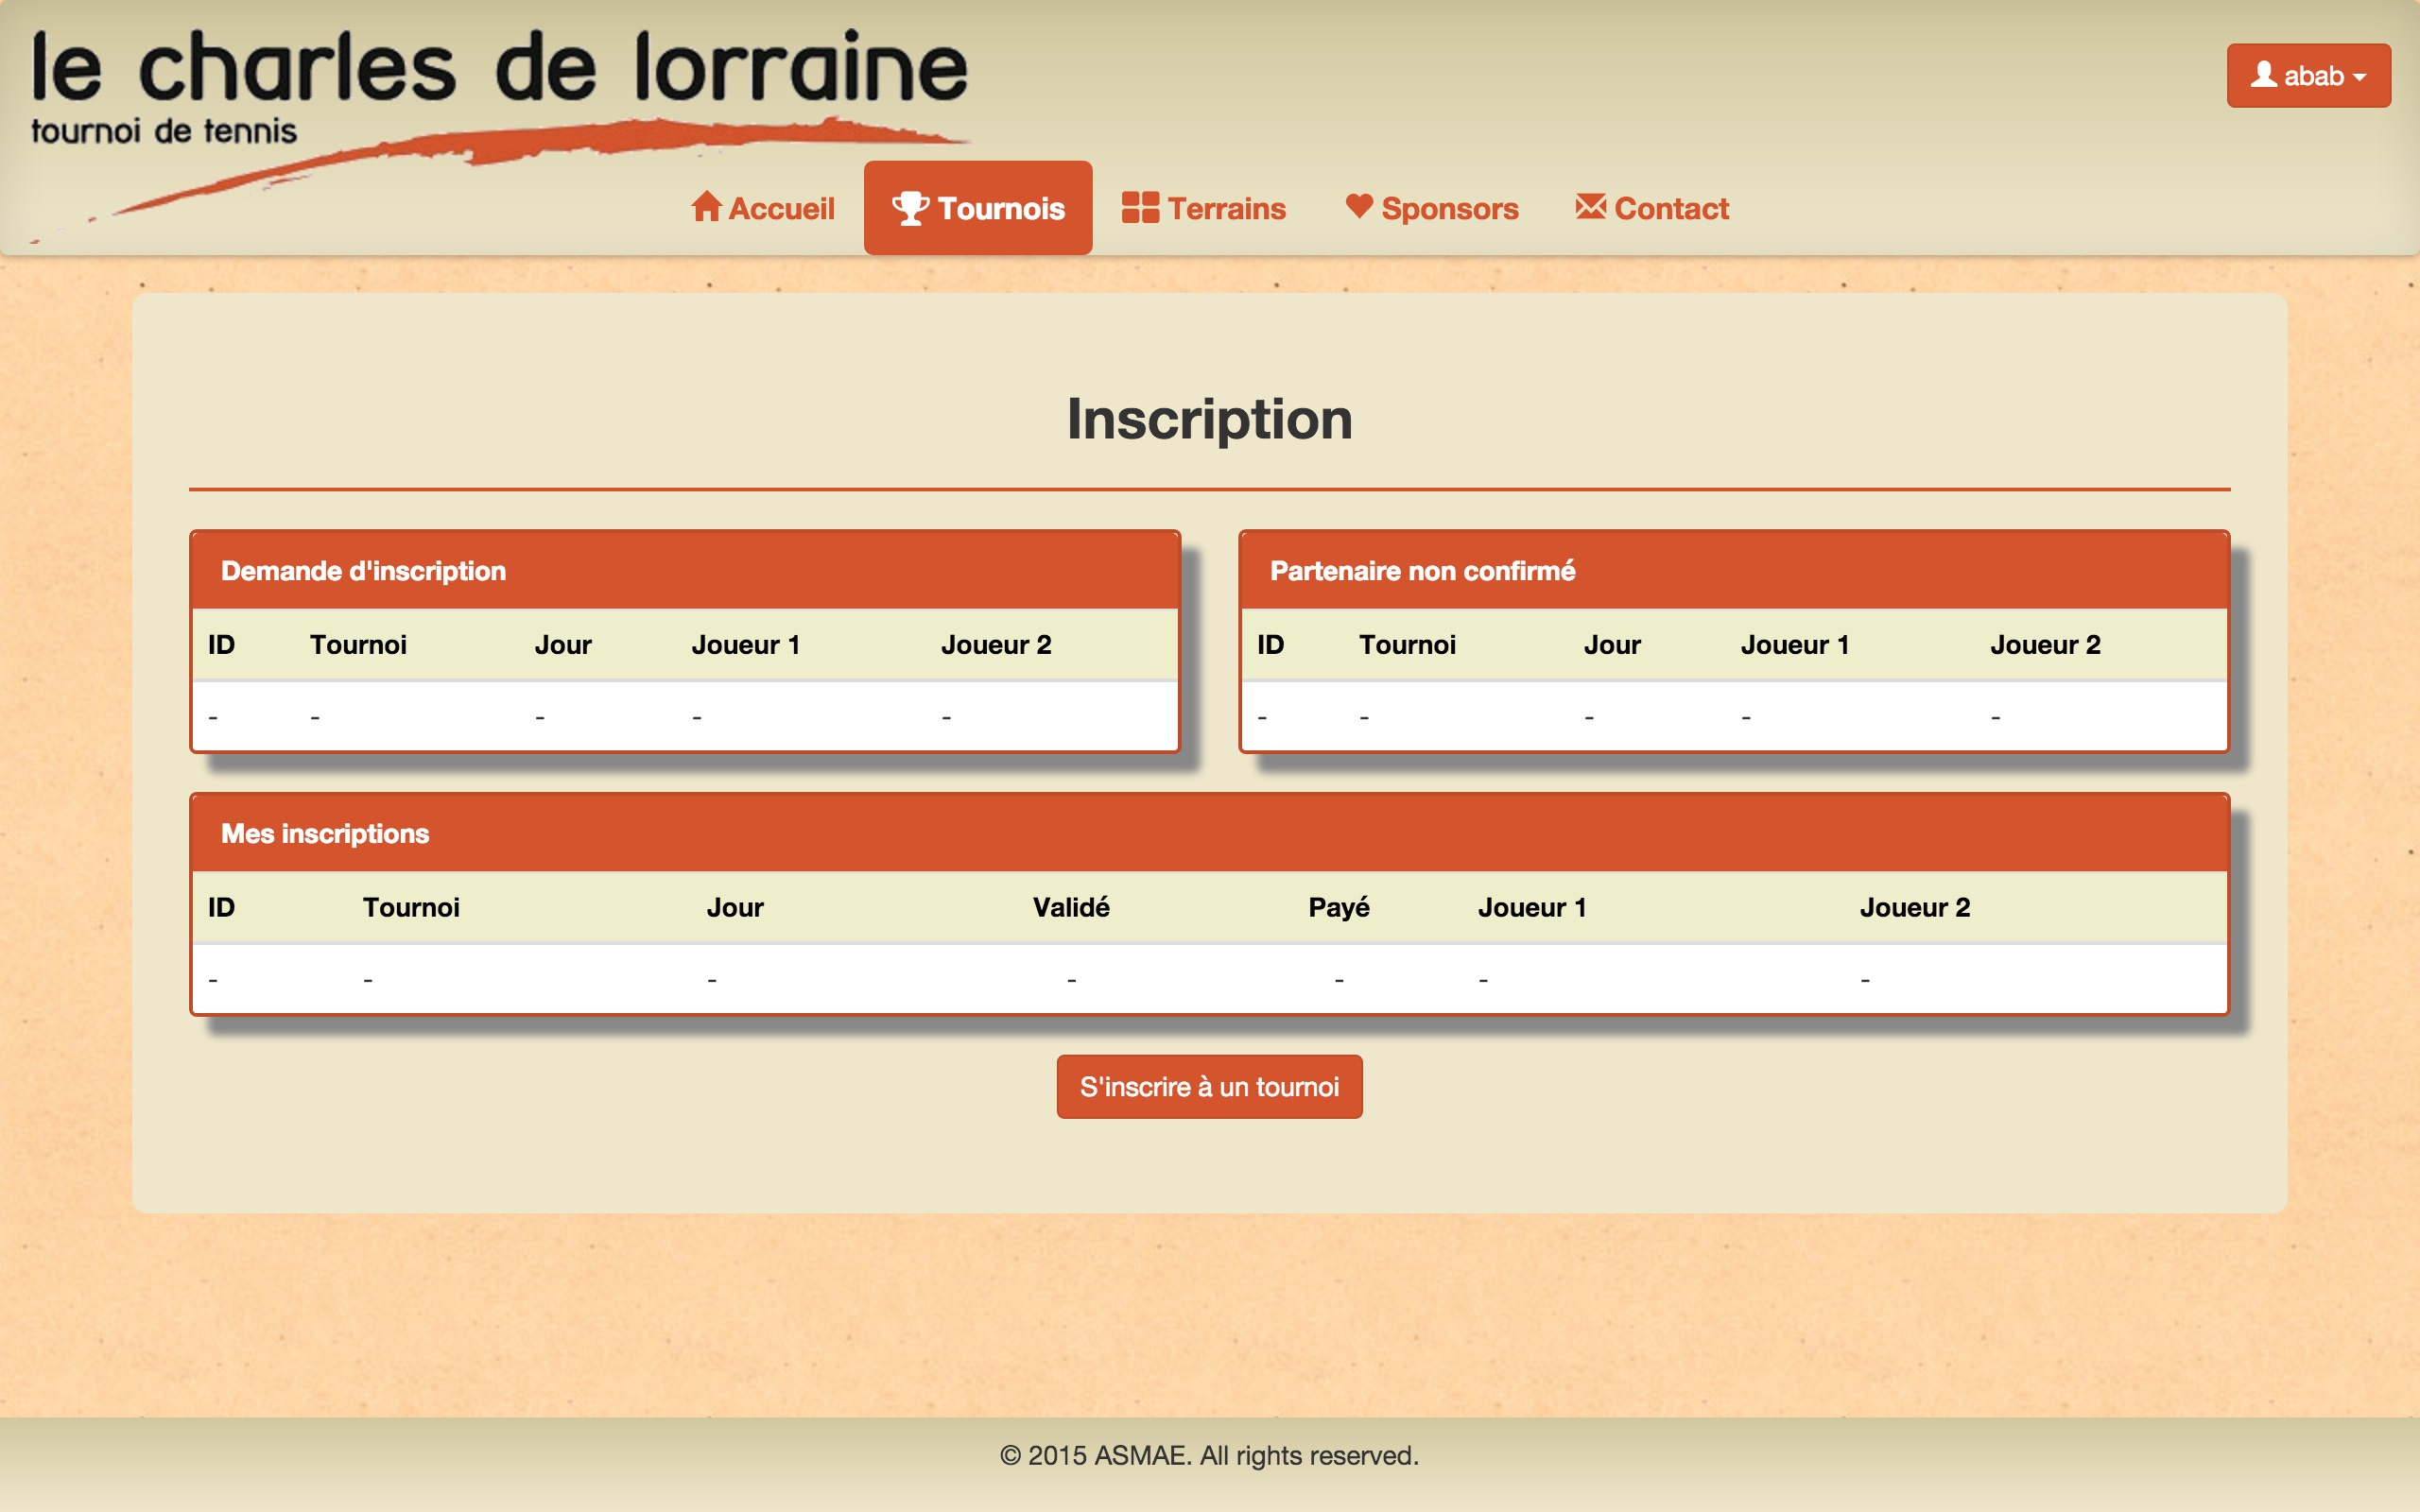
\includegraphics[scale=0.20]{user_images/basic_user/GererConnexion/Senregistrer/005.jpg}
\caption{Création compte, étape 5}
\end{figure}

Si vous cliquez sur le lien, ou copiez-collez le lien dans la barre de navigation de votre navigateur web, vous accéderez à une page qui vous confirme la validation de votre adresse email.

\begin{figure}[H]
\centering
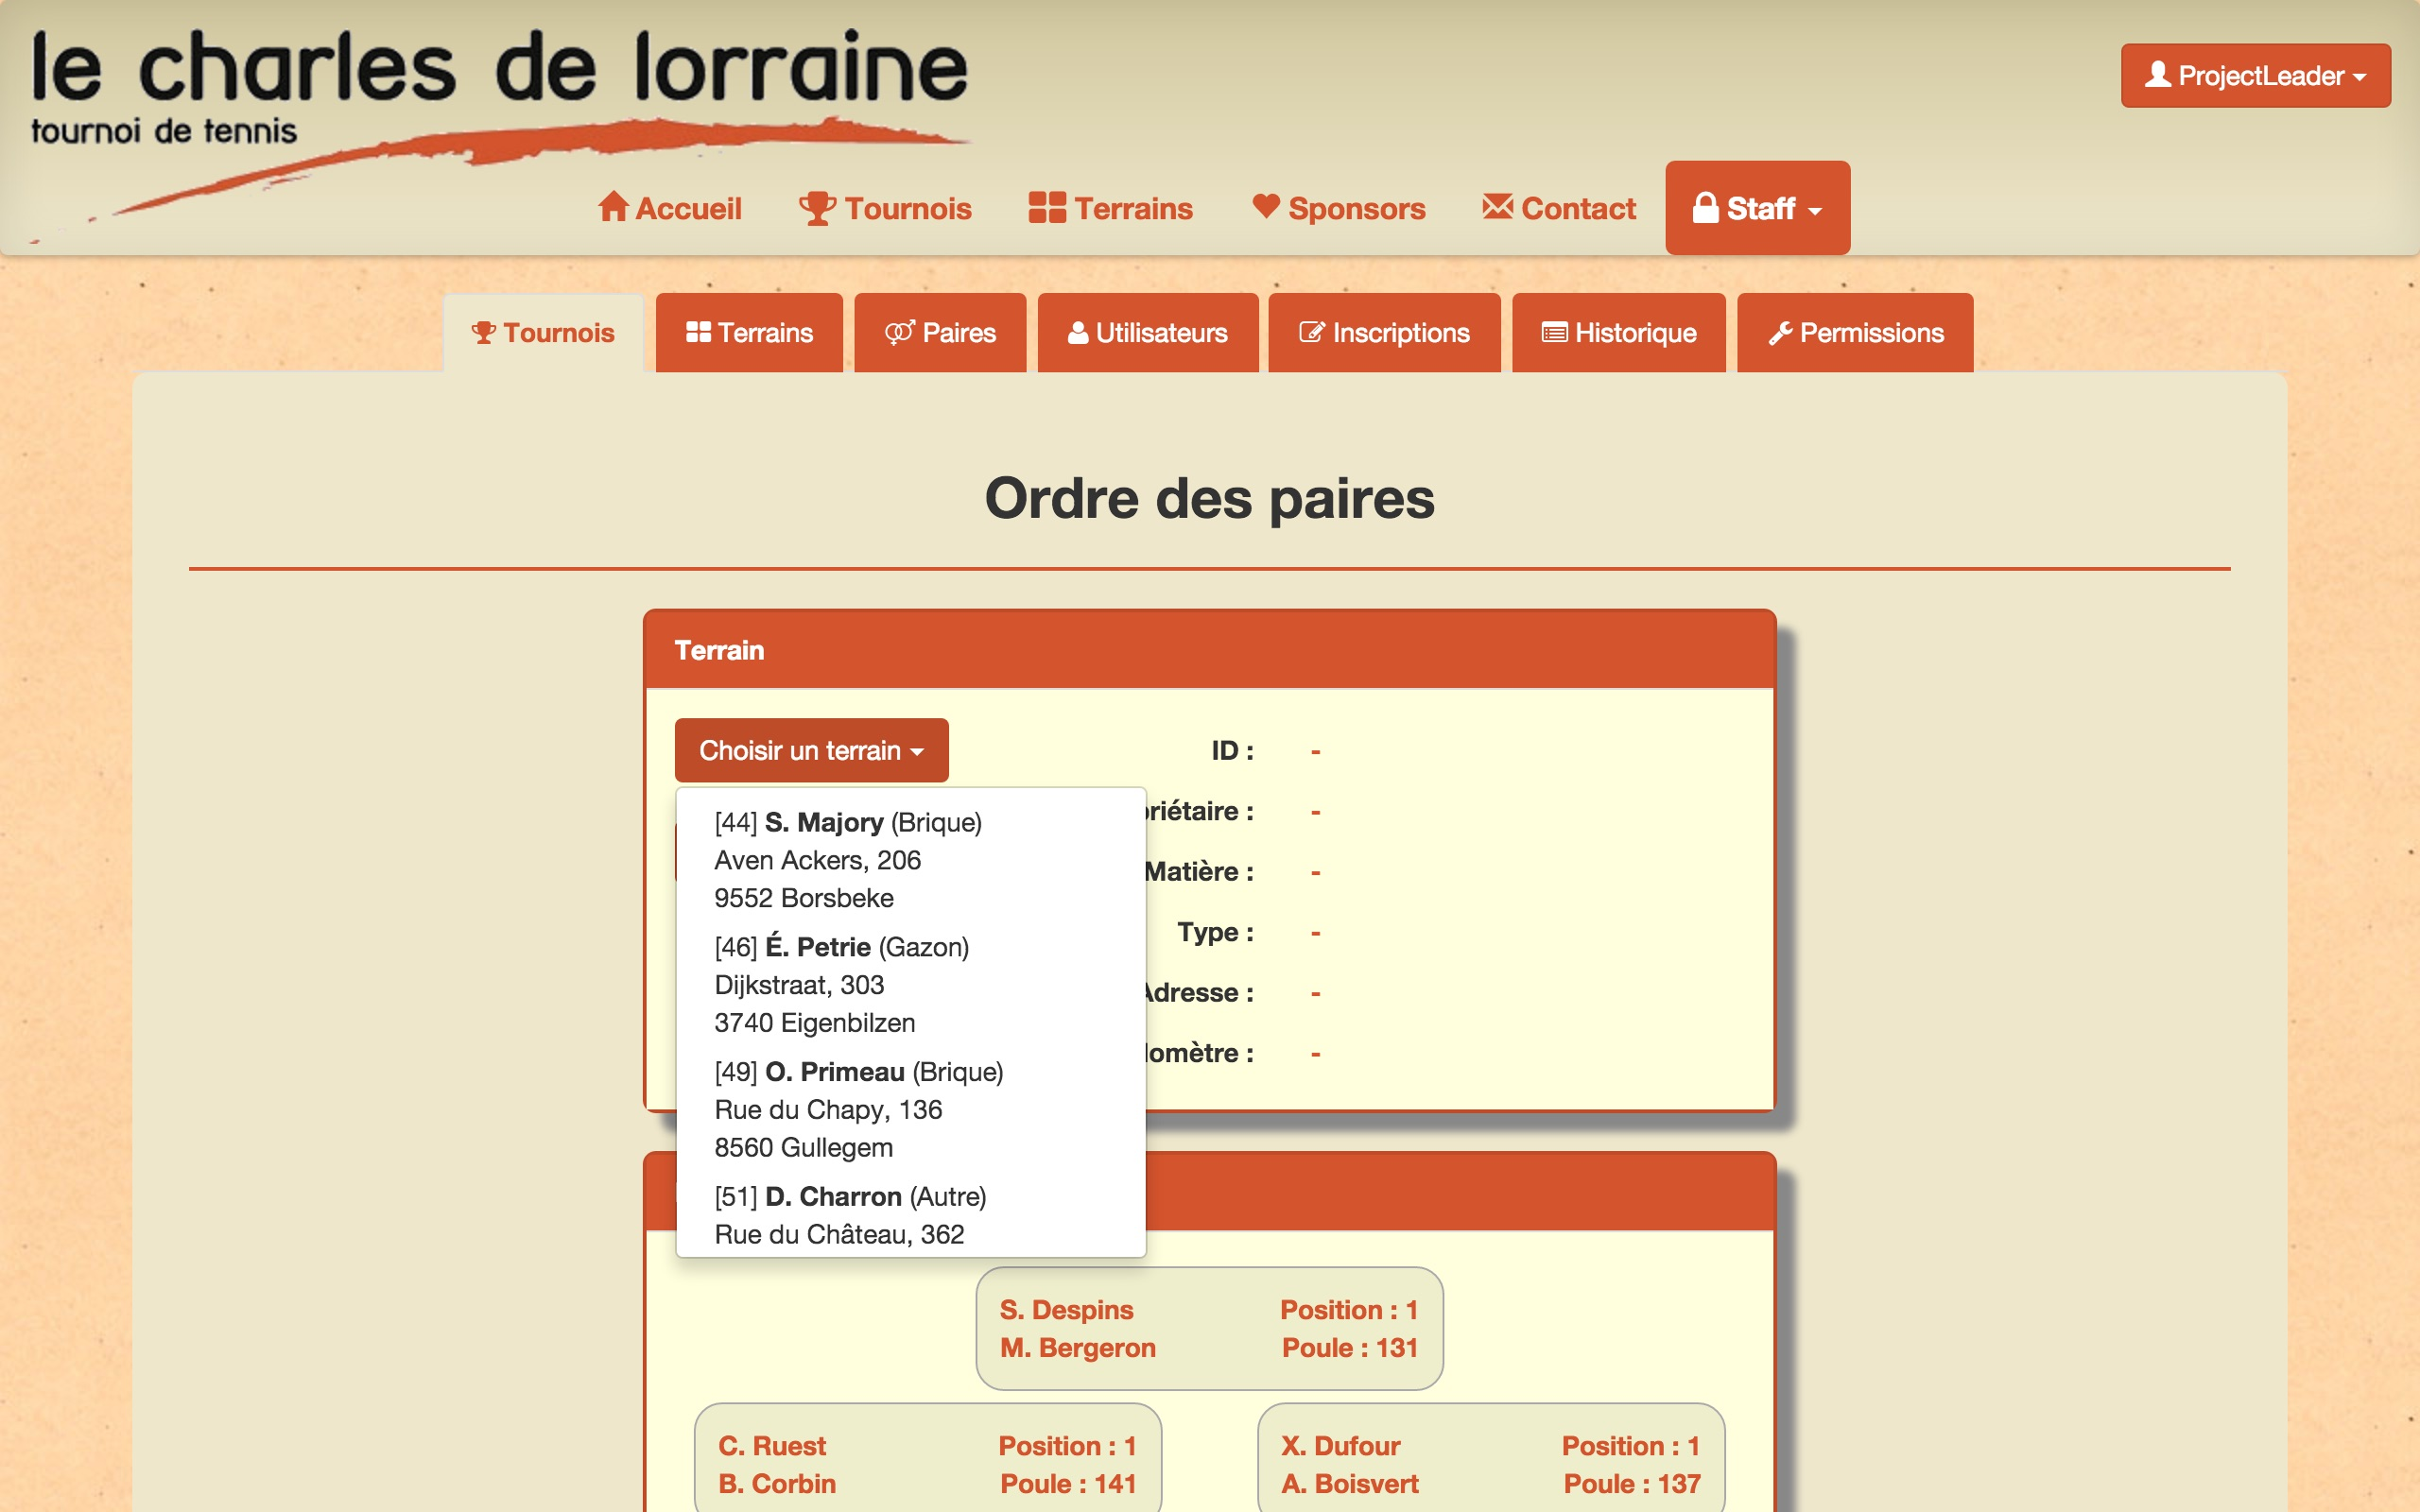
\includegraphics[scale=0.15]{user_images/basic_user/GererConnexion/Senregistrer/006.jpg}
\caption{Création compte, étape 6}
\end{figure}

\subsection{Se connecter}

Pour se connecter avec votre compte, vous devez accéder à la page de connexion, disponible en cliquant sur le bouton "Connexion" dans le menu spécial dans le coin en haut, à droite de n'importe quelle page du site web.

\begin{figure}[H]
\centering
\includegraphics[scale=0.15]{user_images/basic_user/GererConnexion/SeConnecter/001.jpg}
\caption{Se connecter avec son compte, étape 1}
\end{figure}

Sur cette page, vous êtes invités à remplir un formulaire de connexion. Pour s'assurer que le compte vous appartient bien, vous devez fournir le nom du compte et le mot de passe du compte.

\begin{figure}[H]
\centering
\includegraphics[scale=0.15]{user_images/basic_user/GererConnexion/SeConnecter/002.jpg}
\caption{Se connecter avec son compte, étape 2}
\end{figure}

Après avoir rempli ce formulaire, cliquez sur le bouton "Connexion".

\begin{figure}[H]
\centering
\includegraphics[scale=0.15]{user_images/basic_user/GererConnexion/SeConnecter/003.jpg}
\caption{Se connecter avec son compte, étape 3}
\end{figure}

Si le nom du compte et le mot de passe ne sont pas corrects, vous aurez un message d'erreur, vous signalant que le compte et/ou le mot de passe est (sont) éronné(s). Dans le cas contraire, vous serez dirigé vers la page "Tournoi" de l'utilisateur connecté, similairement à l'image ci-dessous.

\begin{figure}[H]
\centering
\includegraphics[scale=0.15]{user_images/basic_user/GererConnexion/SeConnecter/004.jpg}
\caption{Se connecter avec son compte, étape 4}
\end{figure}

\subsection{Récupérer son mot de passe}

Si vous avez oublié votre mot de passe, vous pouvez le récupérer en accédant à la page de connexion.

\begin{figure}[H]
\centering
\includegraphics[scale=0.15]{user_images/basic_user/GererConnexion/RecupMDP/001.jpg}
\caption{Récupération mot de passe, étape 1}
\end{figure}

Au lieu de remplir le formulaire, cliquez sur le bouton "Mot de passe oublié ?".

\begin{figure}[H]
\centering
\includegraphics[scale=0.15]{user_images/basic_user/GererConnexion/RecupMDP/002.jpg}
\caption{Récupération mot de passe, étape 2}
\end{figure}

Sur cette page, un formulaire à un seul champ permet de réinitialiser le mot de passe d'un compte. Pour réinitialiser le mot de passe d'un compte, vous devez fournir l'adresse email du compte que vous souhaitez récupérer.

\begin{figure}[H]
\centering
\includegraphics[scale=0.15]{user_images/basic_user/GererConnexion/RecupMDP/003.jpg}
\caption{Récupération mot de passe, étape 3}
\end{figure}

Dès que vous avez fourni l'adresse email du compte à récupérer, cliquez sur le bouton "Réinitialiser le mot de passe". S'il existe bien un compte avec cette adresse email, un email sera envoyé à cette adresse email, contenant un lien de réinitialisation du mot de passe du compte.

\begin{figure}[H]
\centering
\includegraphics[scale=0.15]{user_images/basic_user/GererConnexion/RecupMDP/004.jpg}
\caption{Récupération mot de passe, étape 4}
\end{figure}

\subsection{Modifier son mot de passe}

Pour modifier le mot de passe de votre compte, vous devez accéder à la page d'édition du profil, accessible via le menu spécial dans le coin en haut, à droite, en cliquant sur "Editer profil".

\begin{figure}[H]
\centering
\includegraphics[scale=0.15]{user_images/basic_user/GererProfil/001.jpg}
\caption{Modifier mot de passe, étape 1}
\end{figure}

Cette page contient les informations du compte et personnelles de l'utilisateur. Le mot de passe est évidemment masqué, pour des raisons de sécurité. Pour modifier le mot de passe, vous devez cliquer sur le bouton "Changer le mot de passe".

\begin{figure}[H]
\centering
\includegraphics[scale=0.15]{user_images/basic_user/GererProfil/ChangerMDP/001.jpg}
\caption{Modifier mot de passe, étape 2}
\end{figure}

Ensuite, vous pouvez modifier le mot de passe en entrant 2 fois le nouveau mot de passe.

\begin{figure}[H]
\centering
\includegraphics[scale=0.15]{user_images/basic_user/GererProfil/ChangerMDP/002.jpg}
\caption{Modifier mot de passe, étape 3}
\end{figure}

Dès que vous avez entré le nouveau mot de passe 2 fois, cliquez sur le bouton "Sauver" pour enregistrer la modification du mot de passe.

\begin{figure}[H]
\centering
\includegraphics[scale=0.15]{user_images/basic_user/GererProfil/ChangerMDP/003.jpg}
\caption{Modifier mot de passe, étape 4}
\end{figure}

\subsection{Modifier ses infos du compte}

Pour modifier les informations personnelles de l'utilisateur, vous devez accéder à la page du profil du compte, comme effectué pour la modification du mot de passe ci-dessus.

\begin{figure}[H]
\centering
\includegraphics[scale=0.15]{user_images/basic_user/GererProfil/EditerInfos/001.jpg}
\caption{Modifier ses infos du compte, étape 2}
\end{figure}

Sur cette page, vous devez cliquer sur le bouton "Editer Info" tout en bas de la page pour accéder à un formulaire d'édition des informations de l'utilisateur.

\begin{figure}[H]
\centering
\includegraphics[scale=0.15]{user_images/basic_user/GererProfil/EditerInfos/002.jpg}
\caption{Modifier ses infos du compte, étape 3}
\end{figure}

Le formulaire est exactement le même que lors de la création du compte, sauf qu'il est pré-rempli avec les informations actuelles. Vous pouvez les modifier à ce moment-là, comme sur l'image ci-dessus. Dès que vous avez terminé avec les modifications, vous pouvez sauvegarder les changements en cliquant sur le bouton "Sauver".

\begin{figure}[H]
\centering
\includegraphics[scale=0.15]{user_images/basic_user/GererProfil/EditerInfos/003.jpg}
\caption{Modifier ses infos du compte, étape 4}
\end{figure}

\subsection{Se déconnecter}

Pour vous déconnecter de votre compte, vous devez cliquer sur "Déconnexion", accessible via le menu spécial du compte dans le coin droit supérieur de n'importe quelle page, comme sur l'image ci-dessous

\begin{figure}[H]
\centering
\includegraphics[scale=0.15]{user_images/basic_user/GererConnexion/SeDeconnecter/001.jpg}
\caption{Récupération mot de passe, étape 1}
\end{figure}

Vous serez bien déconnecté de votre compte, comme le montre le menu spécial de connexion dans le coin droit supérieur : il vous proposera de vous connecter ou de créer un nouveau compte.

\begin{figure}[H]
\centering
\includegraphics[scale=0.15]{user_images/basic_user/GererConnexion/SeDeconnecter/002.jpg}
\caption{Récupération mot de passe, étape 2}
\end{figure}
